\section{T : ADTs - Trees}
\label{chap:adts_trees}

%%%%%%%%%%%%%%%%%%%%%%%%%%%%%%%%%%%%%%%%%%%%%%%%%%%%%%%%%%%%%

\begin{frame}[fragile]
\frametitle{ADTs : Binary Trees}
\begin{columns}[T]

\begin{column}{0.45\textwidth}
\begin{itemize}[<+->]
\item Binary trees are used extensively in computer science	
\item Game Trees	
\item Searching	
\item Sorting	
\end{itemize}	
\pause
\begin{center}
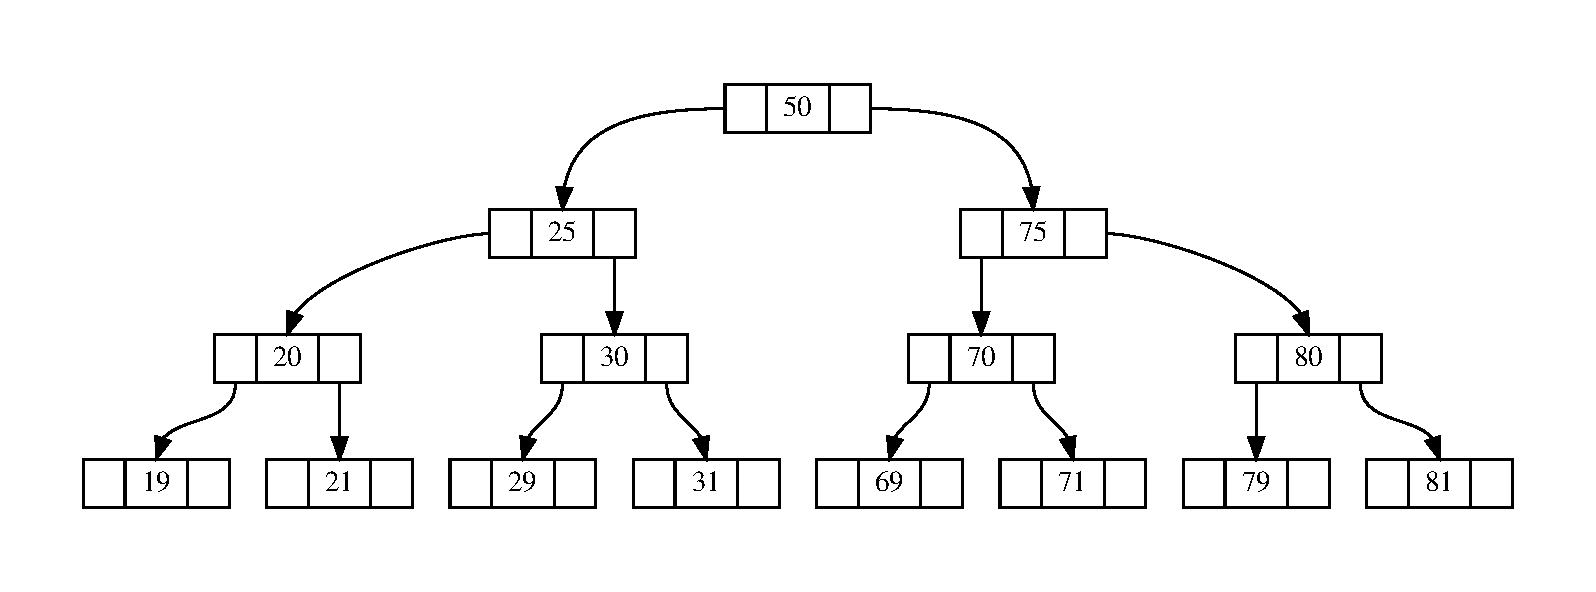
\includegraphics[width=\textwidth]{../Images/Linkedb.pdf}	
\end{center}
\end{column}

\pause
\begin{column}{0.45\textwidth}
\begin{itemize}[<+->]
\item Trees drawn upside-down~!
\item Ancestor relationships: `50' is the parent of~`25' and~`75'.
\item Can refer to left and right children
\item In a tree, there is only one path from the root to any child
\item A node with no children is a leaf
\item Most trees need to be created dynamically
\item Empty subtrees are set to NULL
\end{itemize}
\end{column}

\end{columns}
\end{frame}

%%%%%%%%%%%%%%%%%%%%%%%%%%%%%%%%%%%%%%%%%%%%%%%%%%%%%%%%%%%%%%

\begin{frame}[fragile]
\frametitle{Binary Search Trees}
\begin{columns}[T]

\begin{column}{0.40\textwidth}
In a binary search tree the left-hand tree of a parent contains
all keys less than the parent node, and the right-hand side all
the keys greater than the parent node.	
\begin{center}	
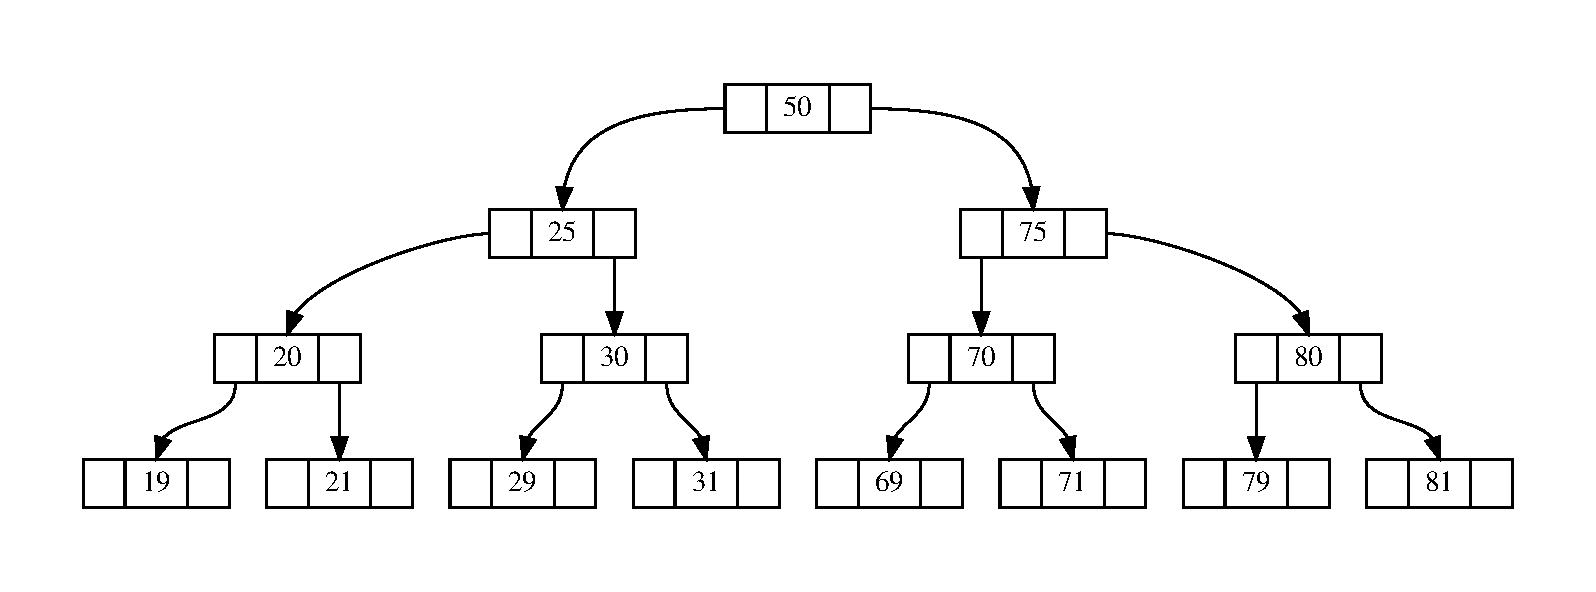
\includegraphics[width=\textwidth]{../Images/Linkedb.pdf}	
\end{center}	
\end{column}

\pause
\begin{column}{0.50\textwidth}
\verb^bst.h^
\lstinputlisting[style=basicc]{../../ADTs/BST/bst.h}
\end{column}

\end{columns}
\end{frame}

%%%%%%%%%%%%%%%%%%%%%%%%%%%%%%%%%%%%%%%%%%%%%%%%%%%%%%%%%%%%%%

\begin{frame}[fragile]
\frametitle{Binary Search Trees : Linked I}
\begin{columns}[T]

\begin{column}{0.45\textwidth}
\verb^specific.h^
\lstinputlisting[style=basicc]{../../ADTs/BST/Linked/specific.h}
\end{column}

\pause
\begin{column}{0.45\textwidth}
%% _insert()
\lstinputlisting[style=basicc,linerange={149-168},numbers=none]{../../ADTs/BST/Linked/linked.c}
\end{column}

\end{columns}
\end{frame}

%%%%%%%%%%%%%%%%%%%%%%%%%%%%%%%%%%%%%%%%%%%%%%%%%%%%%%%%%%%%%%

\begin{frame}[fragile]
\frametitle{Binary Search Trees : Linked II}
\begin{columns}[T]

\begin{column}{0.45\textwidth}
%_isin()
\lstinputlisting[style=basicc,linerange={170-185},numbers=none]{../../ADTs/BST/Linked/linked.c}
\end{column}

\pause
\begin{column}{0.45\textwidth}
%_printlisp()
\lstinputlisting[style=basicc,linerange={205-224},numbers=none]{../../ADTs/BST/Linked/linked.c}
\end{column}

\end{columns}
\end{frame}

%%%%%%%%%%%%%%%%%%%%%%%%%%%%%%%%%%%%%%%%%%%%%%%%%%%%%%%%%%%%%%

\begin{frame}[fragile]
\frametitle{Binary Trees using Arrays~?}
\begin{columns}[T]

\begin{column}{0.35\textwidth}
\begin{itemize}[<+->]
\item Don't rush to assume a linked data structure must be used to
implement trees.
\item You could use $1$ cell of an array for the
first node, the next two cells for its children, the next $4$
cells for their children and so on.
\item You need to mark which cells are in use \& which aren't ...
\end{itemize}
\end{column}

\pause
\begin{column}{0.55\textwidth}
Counting from cell $1$, for a tree with $n$ nodes:
\begin{center}	
\begin{tabular}{|l|l|l|}\hline	
To find & Use & Iff\\ \hline	
The root & $A[1]$ & $A$ is nonempty \\	
The left child of $A[i]$ & $A[2i]$ & $2i \leq n$ \\	
The parent of $A[i]$ & $A[i/2]$ & $i > 1$\\	
Is $A[i]$ a leaf~? & True & $2i > n$\\ \hline	
\end{tabular}	
\end{center}	
\end{column}

\end{columns}
\end{frame}

%%%%%%%%%%%%%%%%%%%%%%%%%%%%%%%%%%%%%%%%%%%%%%%%%%%%%%%%%%%%%%

\begin{frame}[fragile]
\frametitle{Binary Search Trees : Realloc}
\begin{columns}[T]

\begin{column}{0.45\textwidth}
\verb^specific.h^
\lstinputlisting[style=basicc]{../../ADTs/BST/Realloc/specific.h}
\end{column}

\pause
\begin{column}{0.45\textwidth}
Using a queue for Level-Order traversal:
\lstinputlisting[style=basicc,linerange={72-86},numbers=none]{../../ADTs/BST/Realloc/realloc.c}
\end{column}

\end{columns}
\end{frame}

%%%%%%%%%%%%%%%%%%%%%%%%%%%%%%%%%%%%%%%%%%%%%%%%%%%%%%%%%%%%%%

\begin{frame}[fragile]
\frametitle{Binary Search Trees : Complexity}

\begin{itemize}[<+->]
\item So, in a nicely balanced tree, insertion, deletion and search are all \verb^O(log n)^.
\item  But: if the root of the tree is not well chosen, or the keys to be inserted are ordered, the tree can become a linked list~!
\item In this case,  complexity becomes \verb^O(n)^.	
\item The tree search performs best when well balanced trees are formed.
\item Large body of literature about creating \& re-balancing trees - Red-Black trees, Tries, 2-3 trees, AVL trees etc.
\end{itemize}

\end{frame}

%%%%%%%%%%%%%%%%%%%%%%%%%%%%%%%%%%%%%%%%%%%%%%%%%%%%%%%%%%%%%%

\begin{frame}[fragile]
\frametitle{Binary Trees : Huffman Compression I}
\begin{columns}[T]

\begin{column}{0.45\textwidth}
\begin{itemize}[<+->]
\item Often we wish to compress data, to reduce storage requirements, or to speed transmission.
\item  Text is particularly suited to compression since using one byte per character is wasteful - some letters occur much more frequently.
\item  Need to give frequently occurring letters short codes, typically a few bits. Less common letters can have long bit patterns.
\end{itemize}
\end{column}

\begin{column}{0.45\textwidth}
\begin{itemize}[<+->]
\item To encode the string "BABBAGE":

\vspace*{2ex}
\pause
\begin{center}
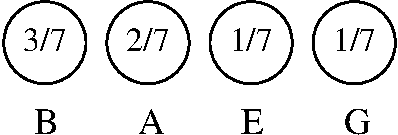
\includegraphics[width=0.6\textwidth]{../Images/huff1.pdf}
\end{center}
\item Keep a list of characters, ordered by their frequency
\end{itemize}
\end{column}

\end{columns}
\end{frame}

%%%%%%%%%%%%%%%%%%%%%%%%%%%%%%%%%%%%%%%%%%%%%%%%%%%%%%%%%%%%%%

\begin{frame}[fragile]
\frametitle{Binary Trees : Huffman Compression II}
\begin{columns}[T]

\begin{column}{0.45\textwidth}
\begin{itemize}[<+->]
\item Use the two least frequent to form a sub-tree, and re-order (sort) the nodes~:

\pause
\vspace*{2ex}
\begin{center}
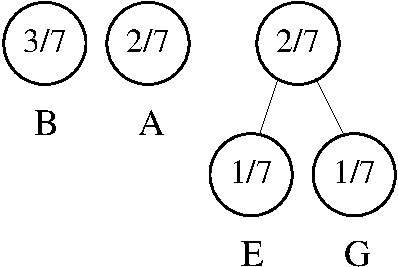
\includegraphics[width=0.6\textwidth]{../Images/huff2.pdf}
\end{center}
\end{itemize}
\end{column}

\pause
\begin{column}{0.45\textwidth}
\begin{center}
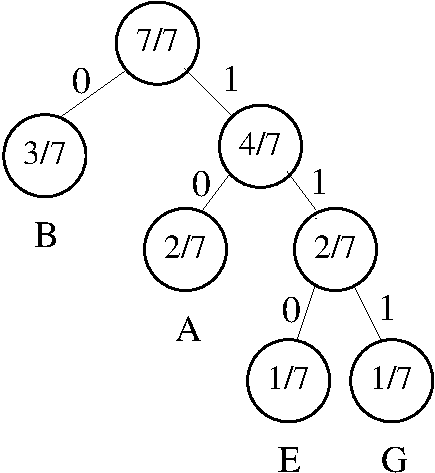
\includegraphics[width=0.6\textwidth]{../Images/huff3.pdf}
\end{center}
\pause
\begin{itemize}[<+->]
\item A = 10, B = 0, E = 110, G = 111
\item String stored using 13 bits.
\end{itemize}
\end{column}

\end{columns}
\end{frame}
